\chapter{КОМПОНЕНТНАЯ БАЗА}
\section{Введение}
\textit{Дописать с соответствием с ТЗ в 1.4}

В выборе компонентной базы мы будем руководствоваться следующими параметрами:
\begin{itemize}
\item простота интеграции;
\item дешевизна;
\item эргономичность.
\end{itemize}

\section{Контроллер}
Если выбирать один контроллер, то он должен поддерживать инитерфейс USB, SPI, иметь достаточное количество цифровых и аналоговых входов/выходов(в соответствии с предведущей главой см.рис.\ref{fig:graf:AppShcSys} на страницена странице \pageref{fig:graf:AppShcSys}), а кроме частота тактирования должна быть достаточно, чтобы поддерживать VGA интерфейс. На рынке есть процессор Atmel SAM3X8E ARM Cortex-M3 на его базе плата DUE V1.6 от Elecfreaks(см. рис.\ref{fig:DueBoard}) с следующими характеристиками см. табл.\ref{tab:DueBoard}\cite{s_1}.
\begin{figure}[ht]
	\centering
     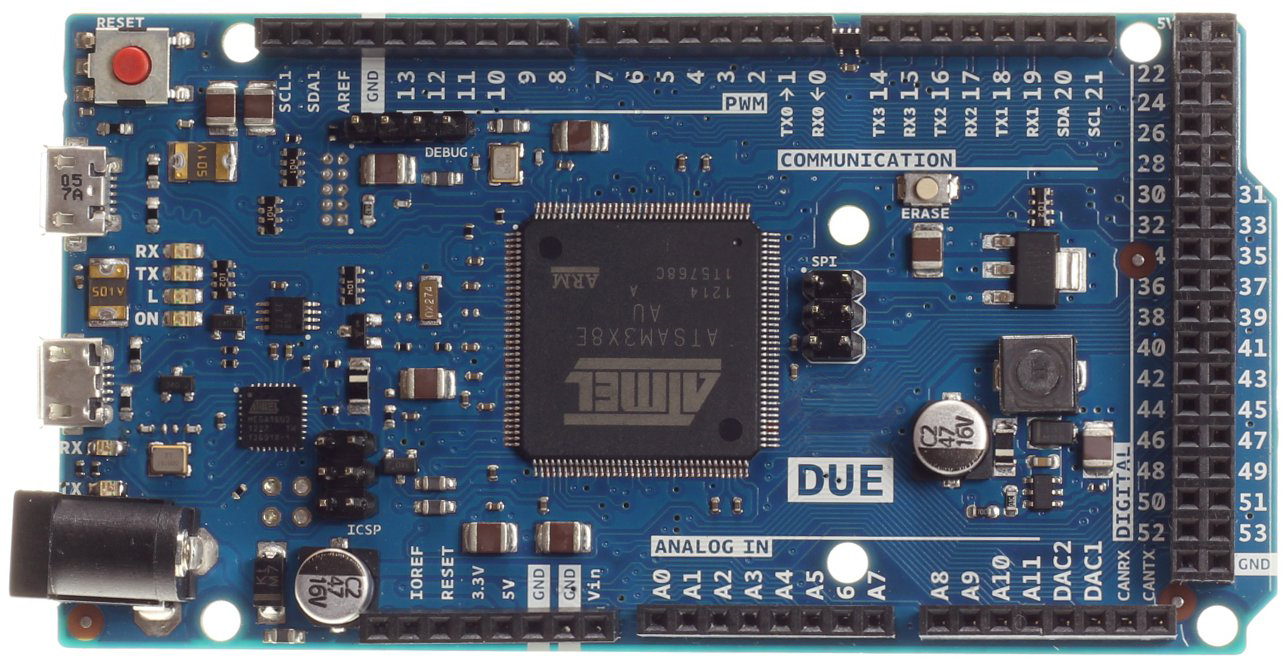
\includegraphics[scale=0.3]{due_board.jpg}
	\caption{Фотография платы.}
	\label{fig:DueBoard}
\end{figure}
\begin{table}
\centering
\begin{tabular}{|c|c|}
\hline 
Микроконтроллер & AT91SAM3X8E \\ 
\hline 
Рабочее напряжение & 3,3 В \\ 
\hline 
Входное напряжение (рекомендуемое) & 7-12 В \\ 
\hline 
Входное напряжение (предельное) & 6-20 В \\ 
\hline 
Цифровые Входы/Выходы & 54 \\ 
\hline 
Аналоговые входы & 12 \\ 
\hline 
Аналоговые выходы & 2 (ЦАП) \\ 
\hline 
Общий выходной постоянный ток & 50 мА \\ 
\hline 
Постоянный ток через вывод 3,3 В & 800 мА \\ 
\hline 
Постоянный ток через вывод 5 В & 800 мА \\ 
\hline 
Флеш-память & 512 КБ \\ 
\hline 
ОЗУ & 96 КБ(64 КБ и 32 КБ)\\ 
\hline 
Тактовая частота & 84 МГц \\ 
\hline 
\end{tabular} 
\caption{Характеристики платы.}
\label{tab:DueBoard}
\end{table}
На плате DUE V1.6 имеется 54 цифровых вход/выхода, 12 аналоговых входов, 4 UARTа (аппаратных последовательных порта), a генератор тактовой частоты 84 МГц, связь по USB с поддержкой OTG, 2 ЦАП (цифро-аналоговых преобразователя), 2 TWI, разъем питания,  разъем SPI, разъем JTAG, кнопка сброса и кнопка стирания. Так же 12 аналоговых входов, каждый из которых может обеспечить разрешение 12 бит (т.е. 4096 различных значений).

Так как эта линейка контроллеров от Elecfreaks очень популярна, DUE V1.6 выпускается большими сериями и дешевле конкурентов, кроме того, для него существует масса библиотек и сопутствующих технических решений, которые позволяют уменьшить срок выхода на рынок и повысить ремонтопригодность. Надо заметим простоту интеграции в разработку благодаря проекту ''DueVGA'' с открытым кодом на сайте распределённой системы управления версиями GitHub\cite{s_2}. Этот проект имеет уже готовую библиотеку для работы с видео интерфейсом VGA. Остановим выбор на этом контроллере.

\section{Привод}
\textit{Когда появится приложение создать ссылку на даташиты шаговых двигателей, если будет достаточно старниц объединить фотографии шагового двигателя, драйвера и модуля драйвера}

Привод должен не только выполнять задачу передачи вращающего момента, то так же чтобы упростить модуль позиционирования тест-объекта, имеет смысл использовать двигатель с управляемым углом поворота. Оно из лучших решений данной задачи - это шаговый двигатель. Большую часть рынка занимают гибридные 2-х/3-х/5-ти фазные шаговые двигатели. Производители заверяют, что погрешность таких двигателей не больше 5\% из-за технологических не совершенств зубцов(точек интенсивных магнитных полей к которым разворачивается ротор).
Имеем следующие параметры системы(см. табл.\ref{tab:MechParamSys})

\begin{table}[ht]
\centering
\begin{tabular}{|c|c|c|c|c|}
\hline 
Скорость передвижения каретки $V$, см/сек & 10\\
\hline 
Радиус передачи момента вращения от вала к ремню $R$, см & 0.5\\
\hline 
Вес каретки $m$, Н & 30\\
\hline 
Коэфициент усилия для передвижения каретки $\theta$ & 1.1\\
\hline 
КПД передачи $\eta$ & 0.9 \\
\hline 

\end{tabular} 
\caption{Параметры системы}
\label{tab:MechParamSys}
\end{table}
Расчет момента удержания шагового двигателя, из уравнения \ref{eq:frec}, из \ref{eq:moment} получим момент вращения вала $M=18.33$ [Н*см].

Из-за физических особенностей шаговых двигателей, крутящий момент двигателя при малых частотах вращения вала примерно равен удерживающему моменту. И наоборот, выходной крутящий момент уменьшается с увеличением частоты вращения вала, так же и выходная мощность, и удерживающий момент становится одним из наиболее важных параметров шагового двигателя. На графике зависимости крутящего момента от частоты вращения для гибридных шаговых двигателей \ref{fig:MomentFrequency} видно, что при частоте $\nu=191$ крутящий момент ослабляется на 15\%, наш привод должен развивать удерживающий момент не меньше $M_{p}=18.3*1.15=21$ [Н*см]
\begin{equation}
\label{eq:frec}
\nu =\frac{V*60}{2*\pi*R}= \frac{10*60}{2*\pi*0.5}=191
\end{equation}

\begin{equation}
\label{eq:moment}
M=\frac{m*\theta*R}{\eta}= \frac{30*1.1*0.005*100}{0.9}=18.33
\end{equation}

\begin{figure}[ht]
	\centering
     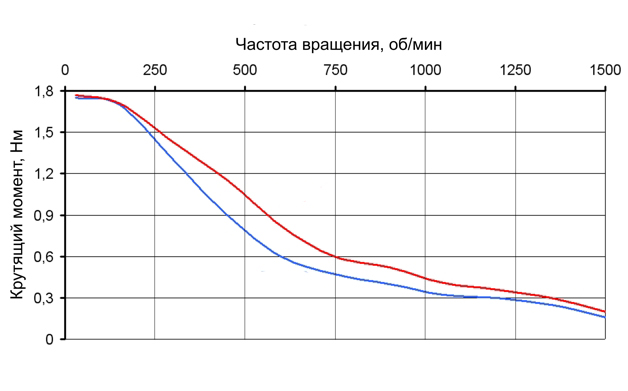
\includegraphics[scale=2.5]{moment_of_frequency_graphic.jpg}
	\caption{График зависимости крутящего момента от частоты вращения шагового двигателя.}
	\label{fig:MomentFrequency}
\end{figure}

Шаговый двигатель 17HS8401(см. рис.\ref{fig:17hs8401_step_motor}) развивает удерживающий крутящий момент $M_{p}=52$ [Н*см], минимальный угол поворота 1.8 градуса, погрешность $\xi=\frac{1.8*0.05*2*\pi*0.5}{360}=8*10^{-3} $[мм]. 17HS8401 применяется в 3D принтерах и как следствие активно используется, имеет отработанные решения, готовые драйверы, это упростит встраивание в наш проект.

\begin{figure}[ht]
	\centering
     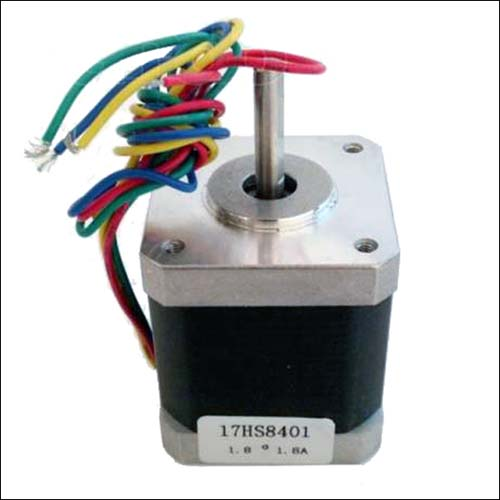
\includegraphics[scale=0.3]{17hs8401_step_motor.jpg}
	\caption{Фотография шагового двигателя.}
	\label{fig:17hs8401_step_motor}
\end{figure}
Драйвер - компонент, цель применение которого упростить подключение шагового двигателя к контроллеру. Напряжение управление не мощным шаговым двигателем обычно в диапазоне от 12 до 48 вольт, а значит перед контроллером необходим усилительный каскад, если не использовать драйвер. Одно из готовых решений для шагового двигателя 17HS8401 - сборка MP1510 с драйвером А4988 (см. рис.\ref{fig:Step_Motor_Driver}).
\begin{figure}[h]
    \centering
    \begin{subfigure}[b]{0.45\textwidth}
    \centering
        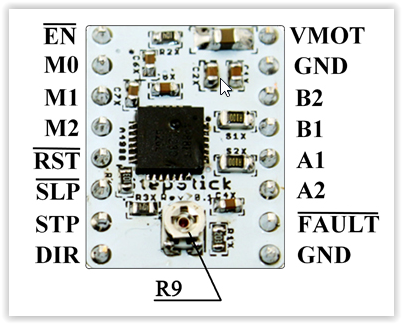
\includegraphics[scale=0.4]{Step_Motor_Driver.PNG}
        \caption{}
    \end{subfigure}
    \begin{subfigure}[b]{0.45\textwidth}
    \centering
        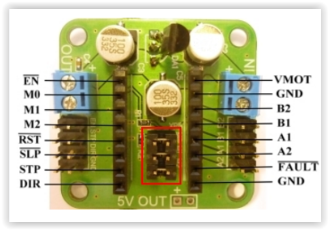
\includegraphics[scale=0.7]{Step_Motor_Driver_Uni_Model.PNG}
        \caption{}
    \end{subfigure}
    \caption{(а) Драйвер шагового двигателя А4988;
    (б) Универсальный модуль подключения драйвера ш.д. MP1510}
    \label{fig:Step_Motor_Driver}
\end{figure}
A4988 и модуль драйвера шагового двигателя(MP1510) содержат набор усилительных каскадов, которые при появлении командного сигнала подают напряжение в 12 вольт на вход двигателя. Контроллер управляет драйвером импульсами напряжения 5 вольт и периодом не меньше 2 мкс.

\section{Концевой выключатель}
Конструкция концевого выключателя (см. рис. \ref{fig:optical_end}, см. табл. \ref{tab:optical_end}) оптимизирована для использования в системах управления:
\begin{itemize}
\item малогабаритный прочный корпус(обычно изготавливаемый из металла) имеет элементы конструкции, позволяющие легко закрепить и сориентировать в пространстве;
\item индикация работы (поданного питания) и срабатывания датчика выполнены при помощи ярких разноцветных светодиодов;
\item подключение производится при помощи общераспространённых однопиновых разъёмов.
\end{itemize}
\begin{table}
	\centering
	\begin{tabular}{|c|c|}
	\hline 
	Оптопара & TCST2103 \\ 
	\hline 
	Номинальный ток, А & 50мА \\ 
	\hline 
	Контактная группа & Фото прерыватель \\ 
	\hline 
	Рабочее напряжение DC, V & 3,2-5 \\ 
	\hline 
	Размеры (HхLхW), мм & 7х32х15 \\ 
	\hline 
	\end{tabular} 
	\caption{Характеристики концевого выключателя}
	\label{tab:optical_end}
\end{table}

\begin{figure}[ht]
	\centering
     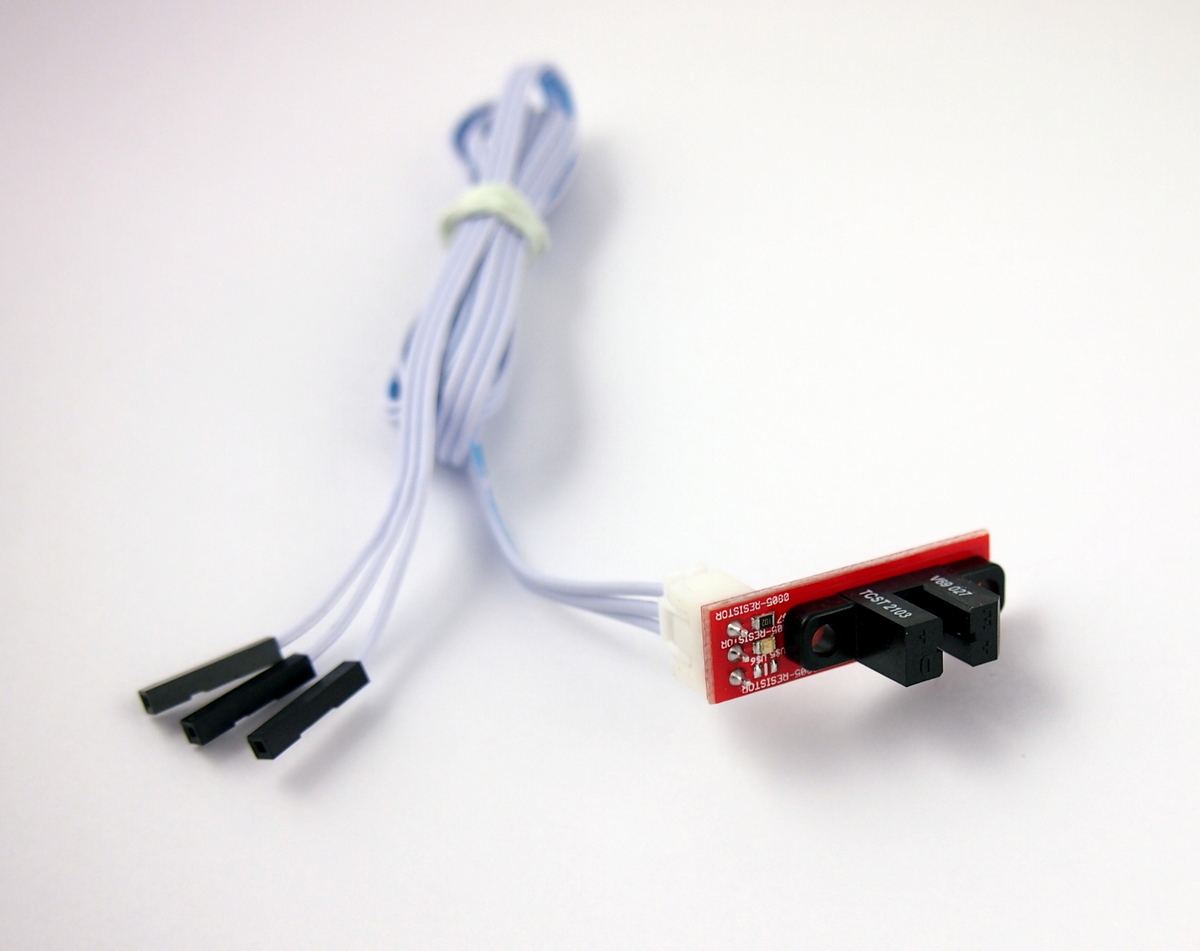
\includegraphics[scale=0.15]{optical_endswitch_with_cable_80cmP1240752.jpg}
	\caption{Оптический ограничитель передвижения каретки.}
	\label{fig:optical_end}
\end{figure}

\section{Датчики определения слайда}
\textit{Когда будет готово ТЗ проверить соответствие опорному числу 20-ти для расчета количества диапозитивов, добавить ссылку на приложение см. момент определения коэф.Стьюдента}

При помещении слайда в каретку система определяет диапозитив, его пространственную ориентацию(см. рис. \ref{fig:slide_orient2}), для этого у каждого слайда должен быть оригинальный идентификационный номер и атрибут по которому можно определить его расположение в каретке. По Т.З. количество диапозитивов не меньше 20-ти.

Размещение по периметру слайда светопроницаемых/частично светопроницаемых/светонепроницаемых ячеек(см. рис. \ref{fig:platform}) дает возможность закодировать идентификационный номер и определить пространственную ориентацию слайда, для считывания ячеек используются оптопары. На одну сторону диапозитива помещается 4 ячейки, размещать ячейки можно только с верху и низу слайда. Частично светопроницаемые ячейки  позволяют использовать многоуровневую(трехуровневую) кодировку.
\begin{figure}[ht]
	\centering
     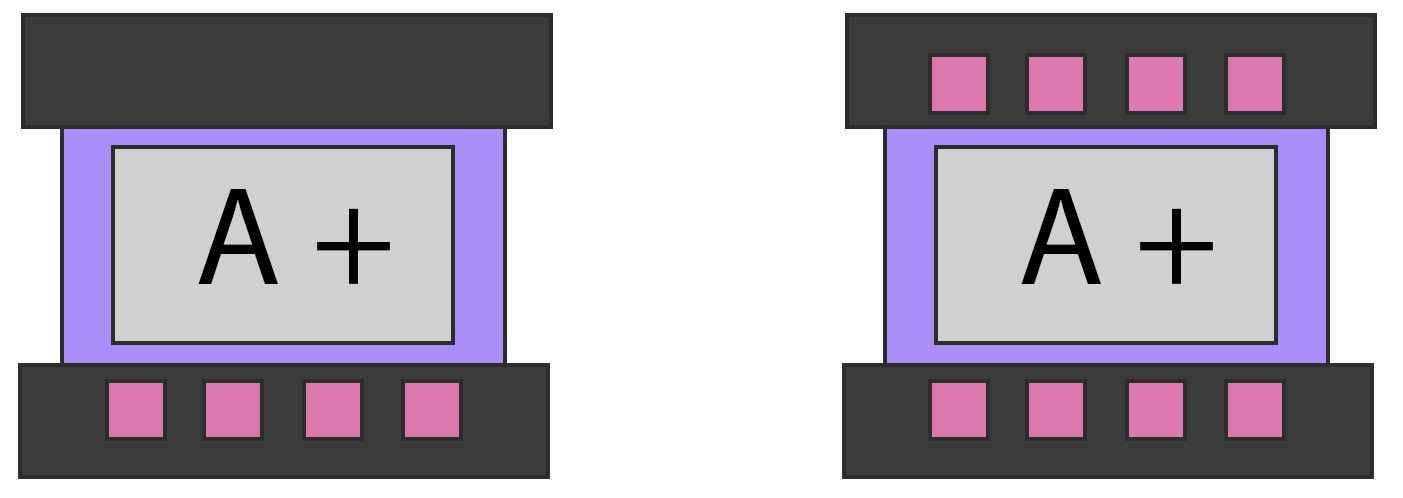
\includegraphics[scale=0.3]{platform.jpg}
	\caption
	{
	Слева одна декодирующая группа каретки(4 оптрона), справа две декодирующие группы каретки(8 оптронов).
	}
	\label{fig:platform}
\end{figure}

\begin{figure}[ht]
	\centering
     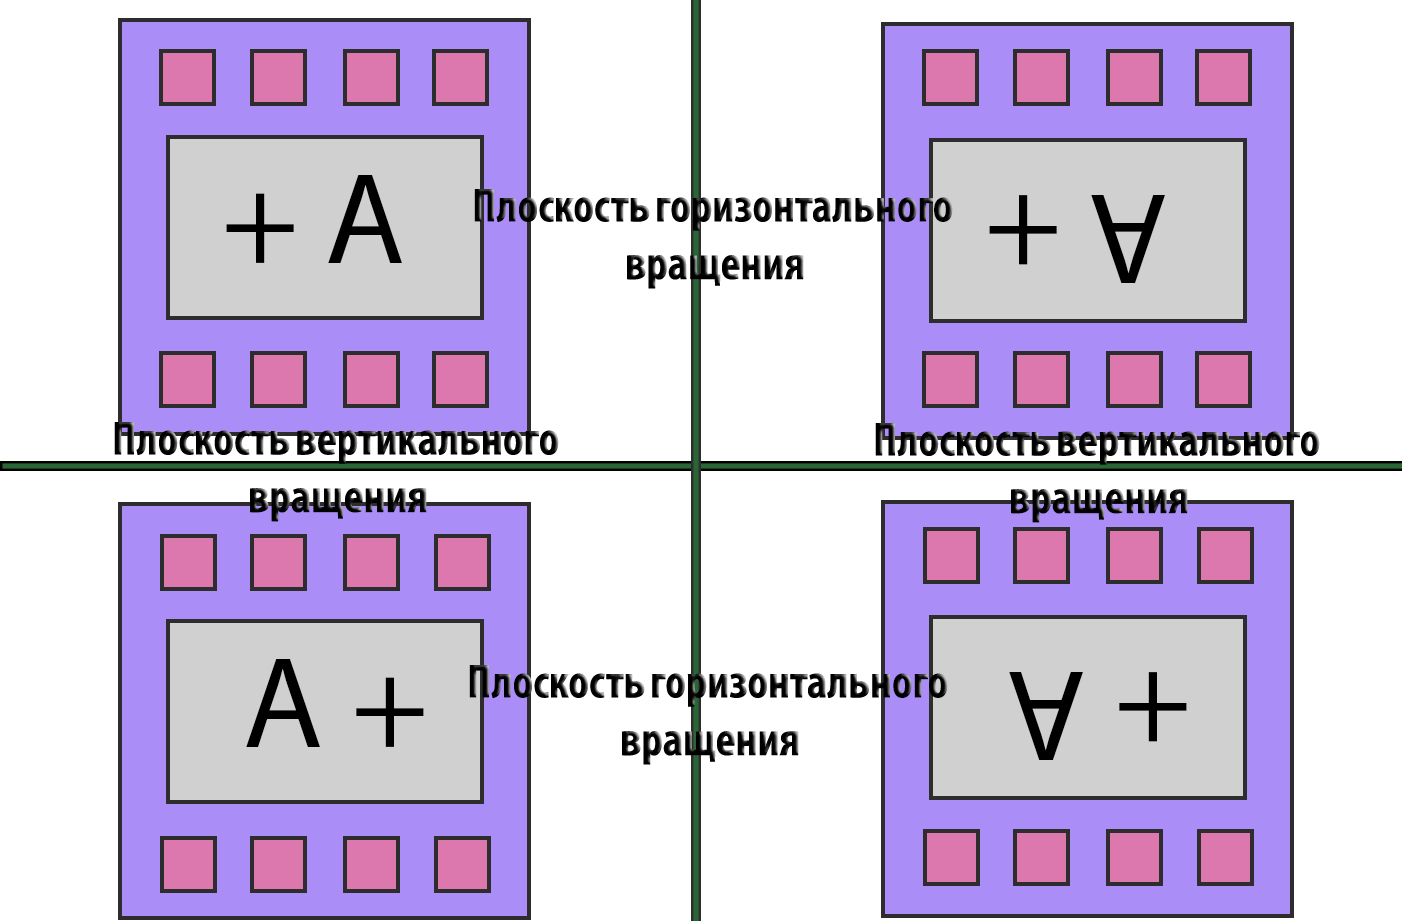
\includegraphics[scale=0.3]{slide_orient2.jpg}
	\caption
	{
	Вращение в двух плоскостях плоскости.
	}
	\label{fig:slide_orient2}
\end{figure}
Рассчитаем количество идентификационных номеров, учитывая, что когда все оптроны получают сигнал не неискаженный ячейками - каретка без слайда.
\begin{itemize}
\renewcommand{\labelitemi}{$\bullet$}
\item для одной декодирующей группы(4 оптрона)
	\begin{itemize}
	\item при вращении в горизонтальной плоскости(см. рис. \ref{fig:slide_orient2})
		\begin{itemize}
			\item для 2-х уровней логики возможно различить 7 слайдов\\
			(комбинаций $2^{4}-1=15$, где $1$-случай когда каретка пуста)
			\item для 3-х уровней логики возможно различить 40 слайдов\\
			(комбинаций $3^{4}-1=80$, где $1$-случай когда каретка пуста)
		\end{itemize}
	\item при вращении в 2-х плоскостях(см. рис. \ref{fig:slide_orient2})
		\begin{itemize}
			\item для 2-х уровней логики возможно различить 2 слайда\\
			(комбинаций $2^{4}-2^{2}=4$, где $2^{2}$-комбинаций не распознаваемых из-за симметрии)
			\item для 3-х уровней логики возможно различить 36 слайдов\\
			(комбинаций $3^{4}-3^{2}=72$, где $3^{2}$-комбинаций не распознаваемых из-за симметрии)
		\end{itemize}
	\end{itemize}
\item для 2-х декодирующих групп(8 оптронов)
	\begin{itemize}
	\item при вращении в горизонтальной плоскости(см. рис. \ref{fig:slide_orient2})
		\begin{itemize}
			\item для 2-х уровней логики возможно различить 127 слайдов\\
			(комбинаций $2^{8}-1=255$, где $1$-случай когда каретка пуста)
		\end{itemize}
	\item при вращении в 2-х плоскостях(см. рис. \ref{fig:slide_orient2})
		\begin{itemize}
			\item для 2-х уровней логики возможно различить 120 слайдов\\
			(комбинаций $2^{8}-2^{4}=240$, где $2^{4}$-комбинаций не распознаваемых из-за симметрии)
		\end{itemize}
	\end{itemize}
\end{itemize}

На следующем снимке осциллографа(см. рис. \ref{fig:optic_oscil}) показано как выходной сигнал с оптрона KTIR0521DS изменяется при изменения светопроницаемой способности кодирующей ячейки.

\begin{figure}[h]
	\centering
     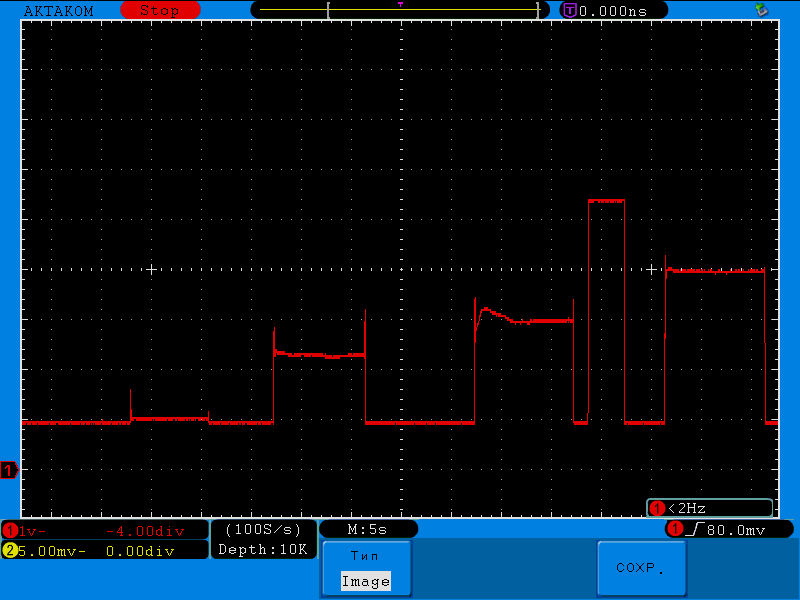
\includegraphics[scale=0.65]{optic_oscil.jpg}
	\caption
	{
	Изменение выходного сигнала оптрона KTIR0521DS при разной светопроницаемой способности кодирующей ячейки.
	}
	\label{fig:optic_oscil}
\end{figure}

Измерениях выходных сигналов для одинаковых степеней проницаемости и разных оптронов KTIR0521DS показали погрешность(см. табл. \ref{tab:optical_error}), средне квадратичная погрешность $ S_{n<X>}=\frac{S_{n}}{\sqrt{n}}=\sqrt{\frac{\sum_{n=0}^\infty(X-<X>)^{2}}{n*(n-1)}}= 0,288$ вольт, тогда для вероятности попадания в доверительный интервал 99\%($t=4.6$ см.таблицу коэффициентов Стьюдента) получим интервал  $ \triangle X = t*S_{n<X>}=1.32$ вольта. Выходной сигнал оптрона находится в диапазоне от 0 до 4.5 вольт, следовательно мы можем использовать трехуровнивую систему кодировки - 40 различимых вариантов диапозитивов.
\begin{table}
	\centering
\begin{tabular}{|c|c|c|c|c|c|}
\hline 
Оптрон & 1 & 2 & 3 & 4 & 5 \\ 
\hline 
Погрешность, В & 0,3 & 0,4 & 0,1 & 0,7 & 0,5 \\ 
\hline 
\end{tabular} 
	\caption{Погрешности разных оптронов KTIR0521DS.}
	\label{tab:optical_error}
\end{table}

\section{Датчик угла поворота}
%\textit{}
%
Инкрементальный датчик угла поворота(энкодер), в проекте его основная задача - дублировать основную систему управления кареткой со стороны администратора, на тот случаи, если такое управление окажется субъективно удобным. Энкодер должен будет иметь не менее 20 импульсов поворота на 360 градусов для плавности управления.

Датчик угла поворота PEC16-4220F-S0024(см. рис. \ref{fig:PEC16-4220F-S0024}) имеет 24 импульсов поворота на круг, кодирование сигнала передается по 2 битам в коде грея, напряжение питания 5 вольт. С точки зрения конструкции у этого энкодера есть необходимая крепежная штанга. Устройство дешево и долговечно.

\begin{figure}[ht]
	\centering
     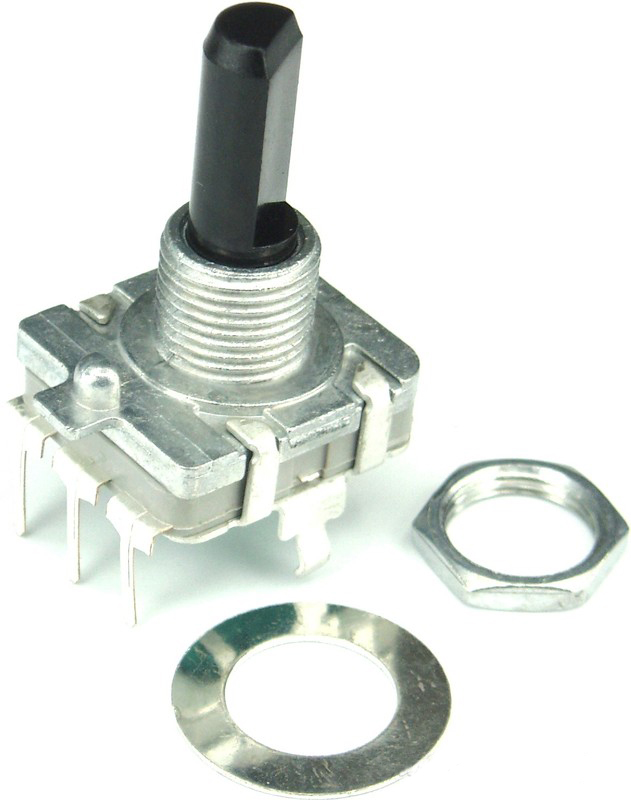
\includegraphics[scale=0.2]{PEC16-4220F-S0024.jpg}
	\caption
	{
	Датчик угла поворота PEC16-4220F-S0024.
	}
	\label{fig:PEC16-4220F-S0024}
\end{figure}

\section{SD картридер}
В современных SD картах есть два режима работы SD и SPI. Последний рассчитан на 8 разрядные микроконтроллеры или  на те микроконтроллеры у которых нет аппаратной поддержки SD режима. Для подключения SD карты мы будем использовать монтажный модуль SD card reader SPI интерфейса(см. рис. \ref{fig:SDCardF}).
\begin{figure}[ht]
	\centering
     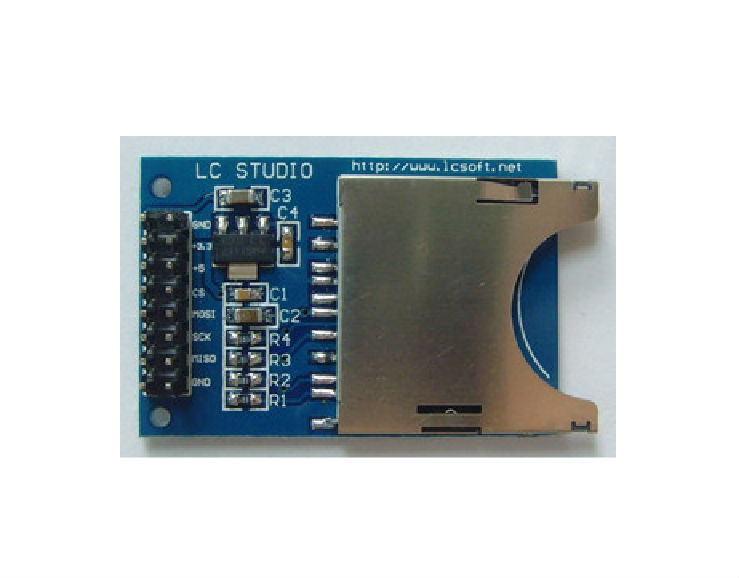
\includegraphics[scale=0.35]{SD-Card-SPI-Mode-SD.jpg}
	\caption
	{
	Монтажный модуль SD картридера.
	}
	\label{fig:SDCardF}
\end{figure}

\section{Джойстик}
Аналоговые джойстики — сенсоры выдающие сигнал значением от нуля до максимума в зависимости от угла отклонения ручки(стика): чем больше рукоять отклонена, тем больше значение напряжения, в пределах опорного. Двумерные джойстики позволяют передавать значения ориентации стика в плоскости. Так же двумерные джойстики могут иметь кнопку, нажатие на которую производится утоплением стика, например(см. рис. \ref{fig:JoystickModuleF}) основанный на 2-х регулируемых делителях напряжения(2 оси задающие ориентацию на плоскости) и ключа(кнопка).
\begin{figure}[ht]
	\centering
     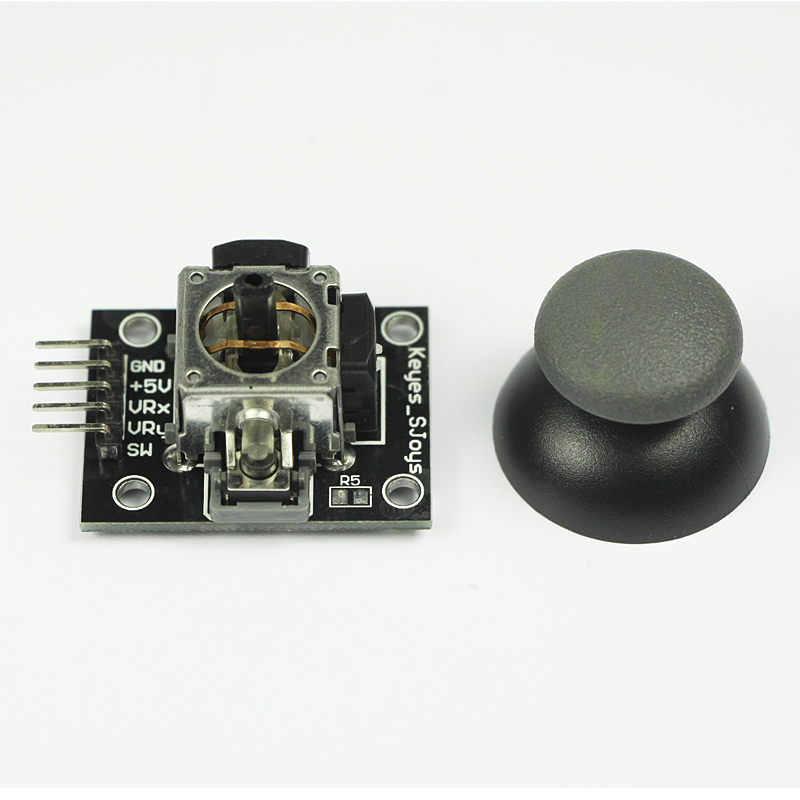
\includegraphics[scale=0.25]{Joystick_Module.jpg}
	\caption
	{
	Монтажный модуль двумерного Джойстика.
	}
	\label{fig:JoystickModuleF}
\end{figure}

\section{Дисплей клиента}
Дисплей играет важную роль вывода информации, дисплей клиента будет не только выводить информацию отображая изображение, а также при вставке слайда его задачей будет освещать необходимый сектора пленки диапозитива. OEL(Organic Electro Luminescent) дисплеи обладают характерной для этих органических матриц высокой насыщенностью, четкостью, яркостью и контрастностью изображения.

Дисплей(см. рис. \ref{fig:OELdisplay}) с разрешением 160 х 128 и цветовой палитрой в 262144 цвета, имеет единственный не достаток - 35 пиновый интерфейс подключения, что в свою очередь замедлит встраивание, но не критично.
\begin{figure}[ht]
	\centering
     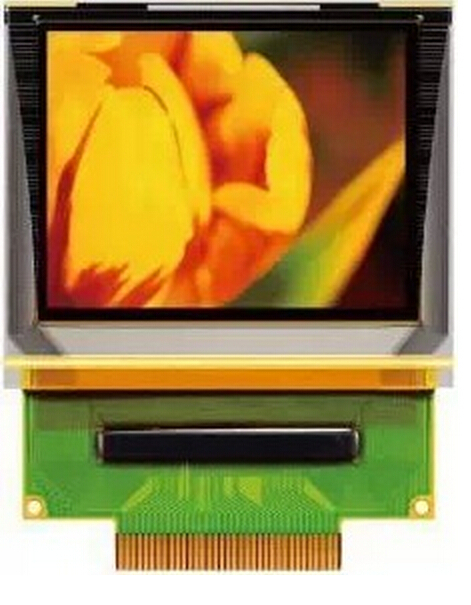
\includegraphics[scale=0.3]{OELdisplay.jpg}
	\caption
	{
	OEL дисплей SAS1-I003-A UG-6028GDEAF01.
	}
	\label{fig:OELdisplay}
\end{figure}

\section{Заключение}
Подведем итоги, выбрана компонентная база(см. табл. \ref{tab:components}) в соответствии с техническим заданием заказчика на основе которой будет построена система управления аппаратом.

\begin{table}[ht]
	\centering
\begin{tabular}{|c|c|}
\hline 
Компонент & Артикул \\ 
\hline 
Контроллер & Due \\ 
\hline 
Шаговый двигатель & 17HS8401 \\ 
\hline 
Концевой выключатель & TCST2103 \\ 
\hline 
Датчики определения слайда & KTIR0521DS \\ 
\hline 
Датчик угла поворота & PEC16-4220F-S0024 \\ 
\hline 
SD картридер & SD Card Module \\ 
\hline 
Джойстик &  KeysSJoys \\ 
\hline 
Дисплей клиента & UG-6028GDEAF01 \\ 
\hline 

\end{tabular} 
	\caption{Таблица компонентов.}
	\label{tab:components}
\end{table}

В следующей главе детально рассмотрим аппаратную часть с приведением электрических схем и принципов их построения, а так же приведем те элементы электроники которые не попали в эту главу.